\documentclass[12pt]{article}
\usepackage[utf8]{inputenc}
\usepackage[T1]{fontenc}
\usepackage{xspace}
\usepackage[french]{babel}
\usepackage{geometry}
\usepackage{graphicx}
\usepackage{float}
\usepackage{caption}
\usepackage{array}

\geometry{hmargin=2.5cm,vmargin=2.5cm}

\title{Rapport Realtime Oscilloscope}
\author{Martin Meyer}
\date{06 Mai 2020}

\begin{document}

	\maketitle
	
	\tableofcontents

	\section{Introduction}
	Dans ce laboratoire, nous avons créé un système temps réel réalisant un fonction d'oscilloscope. Une partie des tâches, comme l'échantillonnage, fonctionne en temps réel. D'autre tâches, comme l'affichage, n'en ont pas besoin.\\
	Pour ce faire, nous avons travaillé avec les cartes microcontrôleur STM32f7-discovery, System Workbench for STM32 et STM32CubeMX.\newline
	Ce rapport décrit quelques parties intéressantes du programme, notamment grâce à des diagrammes UML.
	\section{Tests}
	\subsection{A}
		\begin{table}[H]
			\begin{center}
				\begin{tabular}{| m{2cm}|m{2cm}|m{12cm}|}
					\hline 
					\bf A1&\bf Title:&\bf Check if ADC Signal acquisition is working\\ 
					\hline 
					\multicolumn{2}{|c|}{Group:}&Signal Acquisition\\ 
					\hline 
					\multicolumn{2}{|c|}{Description:}&Is buffer continuously feed with new ADC measures?
					\\ 
					\hline 
					\multicolumn{2}{|c|}{Initial Conditions:}&Running program\\ 
					\hline 
					\multicolumn{2}{|c|}{Test Results:}&The buffer is continuously feed with new ADC measures.\\ 
					\hline 
					\multicolumn{2}{|c|}{Final Conditions:}&Running program\\ 
					\hline 
					\multicolumn{2}{|c|}{Comments:}&\\ 
					\hline 
					\multicolumn{2}{|c|}{Test Passed:}&Yes\\ 
					\hline 
				\end{tabular} 
			\end{center}
		\end{table}
	
		\begin{table}[H]
			\begin{center}
				\begin{tabular}{| m{2cm}|m{2cm}|m{12cm}|}
					\hline 
					\bf A2&\bf Title:&\bf Check TIM1 continously trigger the ADC\\ 
					\hline 
					\multicolumn{2}{|c|}{Group:}&Signal Acquisition\\ 
					\hline 
					\multicolumn{2}{|c|}{Description:}&Not software trigger, nor ADC continous conversion mode\\ 
					\hline 
					\multicolumn{2}{|c|}{Initial Conditions:}&Running program\\ 
					\hline 
					\multicolumn{2}{|c|}{Test Results:}&Yes, the ADC conversion is started directly from the TIM1 timeout signal.\\ 
					\hline 
					\multicolumn{2}{|c|}{Final Conditions:}&Running program\\ 
					\hline 
					\multicolumn{2}{|c|}{Comments:}&\\ 
					\hline 
					\multicolumn{2}{|c|}{Test Passed:}&Yes\\ 
					\hline 
				\end{tabular} 
			\end{center}
		\end{table}	
	
			\begin{table}[H]
		\begin{center}
			\begin{tabular}{| m{2cm}|m{2cm}|m{12cm}|}
				\hline 
				\bf A3&\bf Title:&\bf Check TIM1 trigger frequency\\ 
				\hline 
				\multicolumn{2}{|c|}{Group:}&Signal Acquisition\\ 
				\hline 
				\multicolumn{2}{|c|}{Description:}&Is TIM1 trigger frequency as expected?\\ 
				\hline 
				\multicolumn{2}{|c|}{Initial Conditions:}&-\\ 
				\hline 
				\multicolumn{2}{|c|}{Test Results:}&Test can't be done. No oscilloscope available\\ 
				\hline 
				\multicolumn{2}{|c|}{Final Conditions:}&-\\ 
				\hline 
				\multicolumn{2}{|c|}{Comments:}&\\ 
				\hline 
				\multicolumn{2}{|c|}{Test Passed:}&-\\ 
				\hline 
			\end{tabular} 
		\end{center}
	\end{table}	
	
	%%%%%%%%%%%%%%%%%%%%%%%%%%%%%%%%%%%%%%%%%BBBBBBBBBBBBBBBBBBBBBBBBBBBBBB%%%%%%%%%%%%%%%%%%%%%%%%%%%%%%%%%%%%%%
	\subsection{B}
	\begin{table}[H]
		\begin{center}
			\begin{tabular}{| m{2cm}|m{2cm}|m{12cm}|}
				\hline 
				\bf B1&\bf Title:&\bf Check Sinus wave can be correctly measured\\ 
				\hline 
				\multicolumn{2}{|c|}{Group:}&Signal Frequencies\\ 
				\hline 
				\multicolumn{2}{|c|}{Description:}&50 Hz\\ 
				\hline 
				\multicolumn{2}{|c|}{Initial Conditions:}&Sampling rate : 100kSample/s, Input freq : 50Hz\\ 
				\hline 
				\multicolumn{2}{|c|}{Test Results:}&Test can't be done. No Sinus generator for 50Hz\\ 
				\hline 
				\multicolumn{2}{|c|}{Final Conditions:}&-\\ 
				\hline 
				\multicolumn{2}{|c|}{Comments:}&\\ 
				\hline 
				\multicolumn{2}{|c|}{Test Passed:}&-\\ 
				\hline 
			\end{tabular} 
		\end{center}
	\end{table}	
	\begin{table}[H]
	\begin{center}
		\begin{tabular}{| m{2cm}|m{2cm}|m{12cm}|}
			\hline 
			\bf B2&\bf Title:&\bf Check Sinus wave can be correctly measured\\ 
			\hline 
			\multicolumn{2}{|c|}{Group:}&Signal Frequencies\\ 
			\hline 
			\multicolumn{2}{|c|}{Description:}&370 Hz\\ 
			\hline 
			\multicolumn{2}{|c|}{Initial Conditions:}&Sampling rate : 100kSample/s, Input freq : 370Hz\\ 
			\hline 
			\multicolumn{2}{|c|}{Test Results:}&The sinus is correctly displayed. The input period matches with de divisions\\ 
			\hline 
			\multicolumn{2}{|c|}{Final Conditions:}&-\\ 
			\hline 
			\multicolumn{2}{|c|}{Comments:}&\\ 
			\hline 
			\multicolumn{2}{|c|}{Test Passed:}&Yes\\ 
			\hline 
		\end{tabular} 
	\end{center}
\end{table}	
	\begin{table}[H]
	\begin{center}
		\begin{tabular}{| m{2cm}|m{2cm}|m{12cm}|}
			\hline 
			\bf B3&\bf Title:&\bf Check Sinus wave can be correctly measured\\ 
			\hline 
			\multicolumn{2}{|c|}{Group:}&Signal Frequencies\\ 
			\hline 
			\multicolumn{2}{|c|}{Description:}&500 Hz\\ 
			\hline 
			\multicolumn{2}{|c|}{Initial Conditions:}&Sampling rate : 100kSample/s, Input freq : 500Hz\\ 
			\hline 
			\multicolumn{2}{|c|}{Test Results:}&The sinus is correctly displayed. The input period matches with de divisions\\ 
			\hline 
			\multicolumn{2}{|c|}{Final Conditions:}&\\ 
			\hline 
			\multicolumn{2}{|c|}{Comments:}&\\ 
			\hline 
			\multicolumn{2}{|c|}{Test Passed:}&Yes \\ 
			\hline 
		\end{tabular} 
	\end{center}
\end{table}	
	\begin{table}[H]
	\begin{center}
		\begin{tabular}{| m{2cm}|m{2cm}|m{12cm}|}
			\hline 
			\bf B4&\bf Title:&\bf Check Sinus wave can be correctly measured\\ 
			\hline 
			\multicolumn{2}{|c|}{Group:}&Signal Frequencies\\ 
			\hline 
			\multicolumn{2}{|c|}{Description:}&700 Hz\\ 
			\hline 
			\multicolumn{2}{|c|}{Initial Conditions:}&Sampling rate : 100kSample/s, Input freq : 700Hz\\ 
			\hline 
			\multicolumn{2}{|c|}{Test Results:}&The sinus is correctly displayed. The input period matches with de divisions\\ 
			\hline 
			\multicolumn{2}{|c|}{Final Conditions:}&\\ 
			\hline 
			\multicolumn{2}{|c|}{Comments:}&\\ 
			\hline 
			\multicolumn{2}{|c|}{Test Passed:}&Yes \\ 
			\hline 
		\end{tabular} 
	\end{center}
\end{table}	
	
	%%%%%%%%%%%%%%%%%%%%%%%%%%%%%%%%%%%%%%%%%%%%%%CCCCCCCCCCCCCCCCCCCCCCCCCCCCCCCCCCCCCCCCCCCC
	\subsection{C}
	\begin{table}[H]
		\begin{center}
			\begin{tabular}{| m{2cm}|m{2cm}|m{12cm}|}
				\hline 
				\bf C1&\bf Title:&\bf Check maximum sampling rate\\ 
				\hline 
				\multicolumn{2}{|c|}{Group:}&Maximum Sampling Rate\\ 
				\hline 
				\multicolumn{2}{|c|}{Description:}&Sample singnal with 10 k samples/s\\ 
				\hline 
				\multicolumn{2}{|c|}{Initial Conditions:}&No DMA, Sampling rate: 10kSamples/s\\ 
				\hline 
				\multicolumn{2}{|c|}{Test Results:}&The sampling works\\ 
				\hline 
				\multicolumn{2}{|c|}{Final Conditions:}&\\ 
				\hline 
				\multicolumn{2}{|c|}{Comments:}&\\ 
				\hline 
				\multicolumn{2}{|c|}{Test Passed:}&Yes \\ 
				\hline 
			\end{tabular} 
		\end{center}
	\end{table}	
	\begin{table}[H]
		\begin{center}
			\begin{tabular}{| m{2cm}|m{2cm}|m{12cm}|}
				\hline 
				\bf C2&\bf Title:&\bf Check maximum sampling rate\\ 
				\hline 
				\multicolumn{2}{|c|}{Group:}&Maximum Sampling Rate\\ 
				\hline 
				\multicolumn{2}{|c|}{Description:}&Sample singnal with 100 k samples/s\\ 
				\hline 
				\multicolumn{2}{|c|}{Initial Conditions:}&No DMA, Sampling rate: 100kSamples/s\\ 
				\hline 
				\multicolumn{2}{|c|}{Test Results:}&The sampling works\\ 
				\hline 
				\multicolumn{2}{|c|}{Final Conditions:}&\\ 
				\hline 
				\multicolumn{2}{|c|}{Comments:}&\\ 
				\hline 
				\multicolumn{2}{|c|}{Test Passed:}&Yes \\ 
				\hline 
			\end{tabular} 
		\end{center}
	\end{table}	

		\begin{table}[H]
	\begin{center}
		\begin{tabular}{| m{2cm}|m{2cm}|m{12cm}|}
			\hline 
			\bf C3&\bf Title:&\bf Check maximum sampling rate\\ 
			\hline 
			\multicolumn{2}{|c|}{Group:}&Maximum Sampling Rate\\ 
			\hline 
			\multicolumn{2}{|c|}{Description:}&Sample singnal with 1 M samples/s\\ 
			\hline 
			\multicolumn{2}{|c|}{Initial Conditions:}&No DMA, Sampling rate: 1MSamples/s\\ 
			\hline 
			\multicolumn{2}{|c|}{Test Results:}&The sampling doesn't work. The uC is fully used for the ADC conversion.\\ 
			\hline 
			\multicolumn{2}{|c|}{Final Conditions:}&\\ 
			\hline 
			\multicolumn{2}{|c|}{Comments:}&\\ 
			\hline 
			\multicolumn{2}{|c|}{Test Passed:}&No \\ 
			\hline 
		\end{tabular} 
	\end{center}
\end{table}	
\subsection{D}
		\begin{table}[H]
	\begin{center}
		\begin{tabular}{| m{2cm}|m{2cm}|m{12cm}|}
			\hline 
			\bf D1&\bf Title:&\bf Check if Sinus wave can be correclty visualised\\ 
			\hline 
			\multicolumn{2}{|c|}{Group:}&Signal Display\\ 
			\hline 
			\multicolumn{2}{|c|}{Description:}&50 Hz Signal with 500 us/div time base\\ 
			\hline 
			\multicolumn{2}{|c|}{Initial Conditions:}&Sampling rate: 100kSamples/s\\ 
			\hline 
			\multicolumn{2}{|c|}{Test Results:}&The sampling frequency is high enough. There are enough points.
			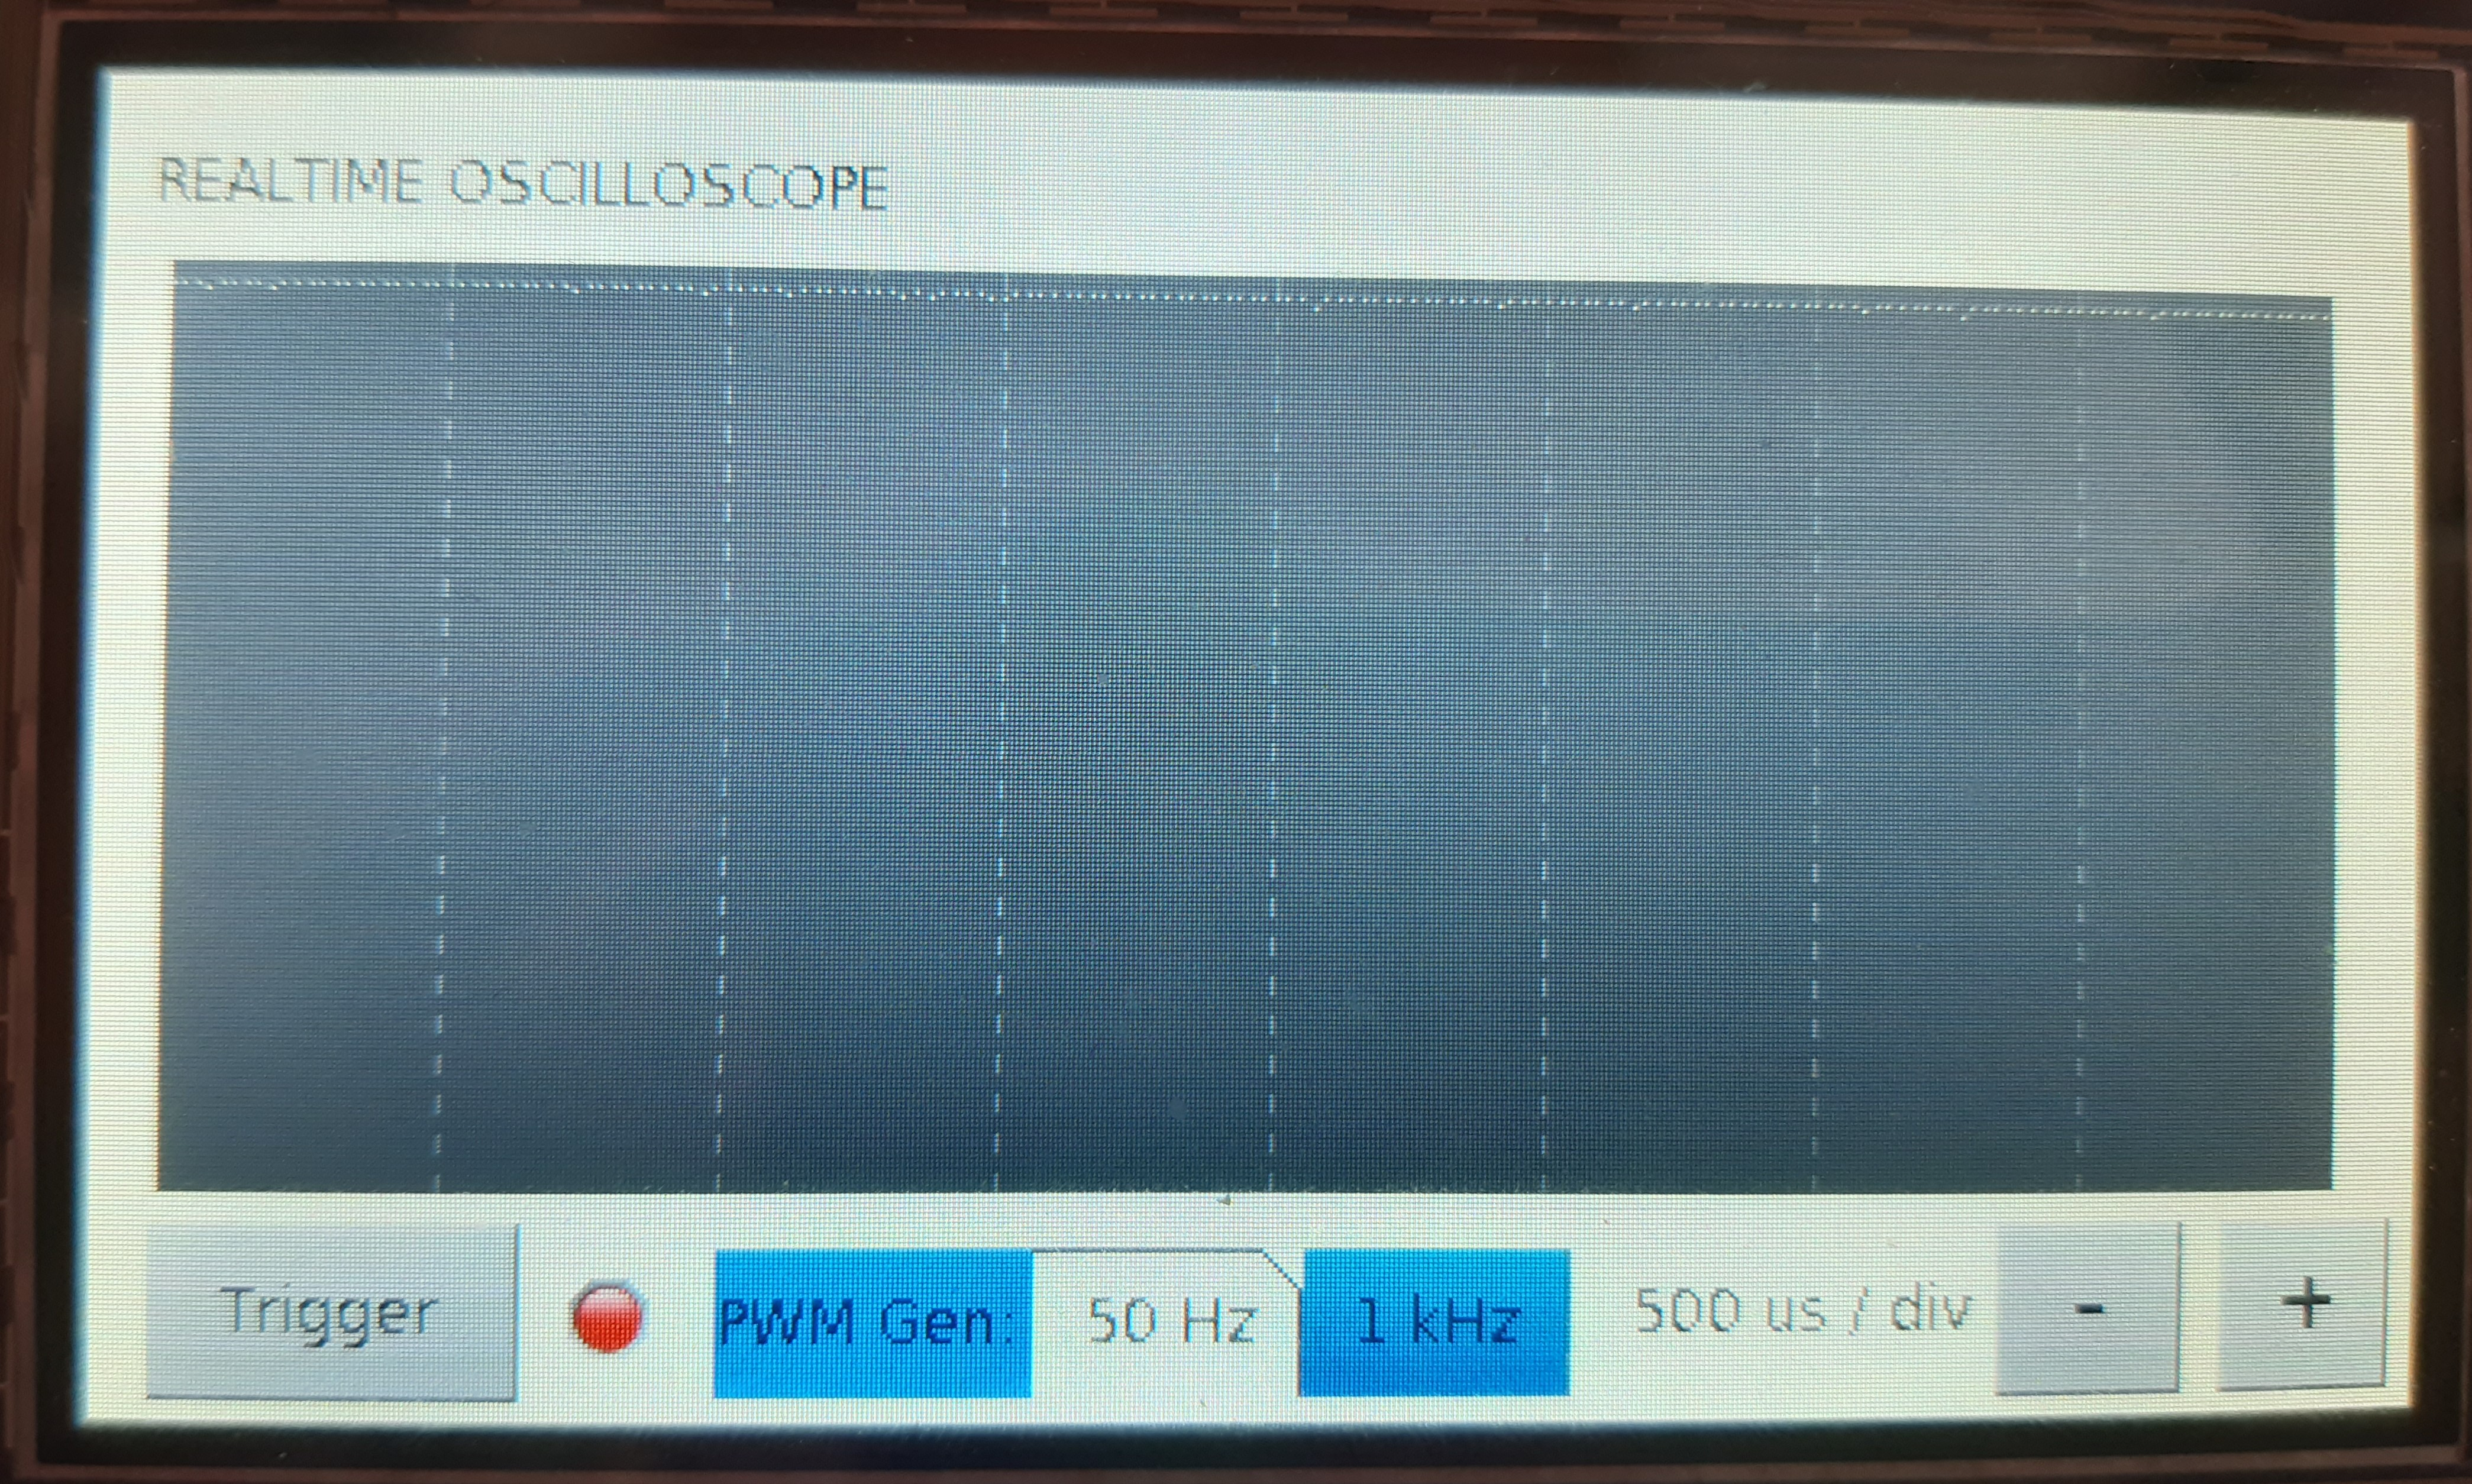
\includegraphics[scale=0.08]{Ressources/PWM_500us}\\ 
			\hline 
			\multicolumn{2}{|c|}{Final Conditions:}&\\ 
			\hline 
			\multicolumn{2}{|c|}{Comments:}&\\ 
			\hline 
			\multicolumn{2}{|c|}{Test Passed:}&Yes \\ 
			\hline 
		\end{tabular} 
	\end{center}
\end{table}	
		\begin{table}[H]
	\begin{center}
		\begin{tabular}{| m{2cm}|m{2cm}|m{12cm}|}
			\hline 
			\bf D2&\bf Title:&\bf Check if Sinus wave can be correclty visualised\\ 
			\hline 
			\multicolumn{2}{|c|}{Group:}&Signal Display\\ 
			\hline 
			\multicolumn{2}{|c|}{Description:}&50 Hz Signal with 10 ms/div time base\\ 
			\hline 
			\multicolumn{2}{|c|}{Initial Conditions:}&Sampling rate: 100kSamples/s\\ 
			\hline 
			\multicolumn{2}{|c|}{Test Results:}&The sampling frequency is high enough. There are enough points.
			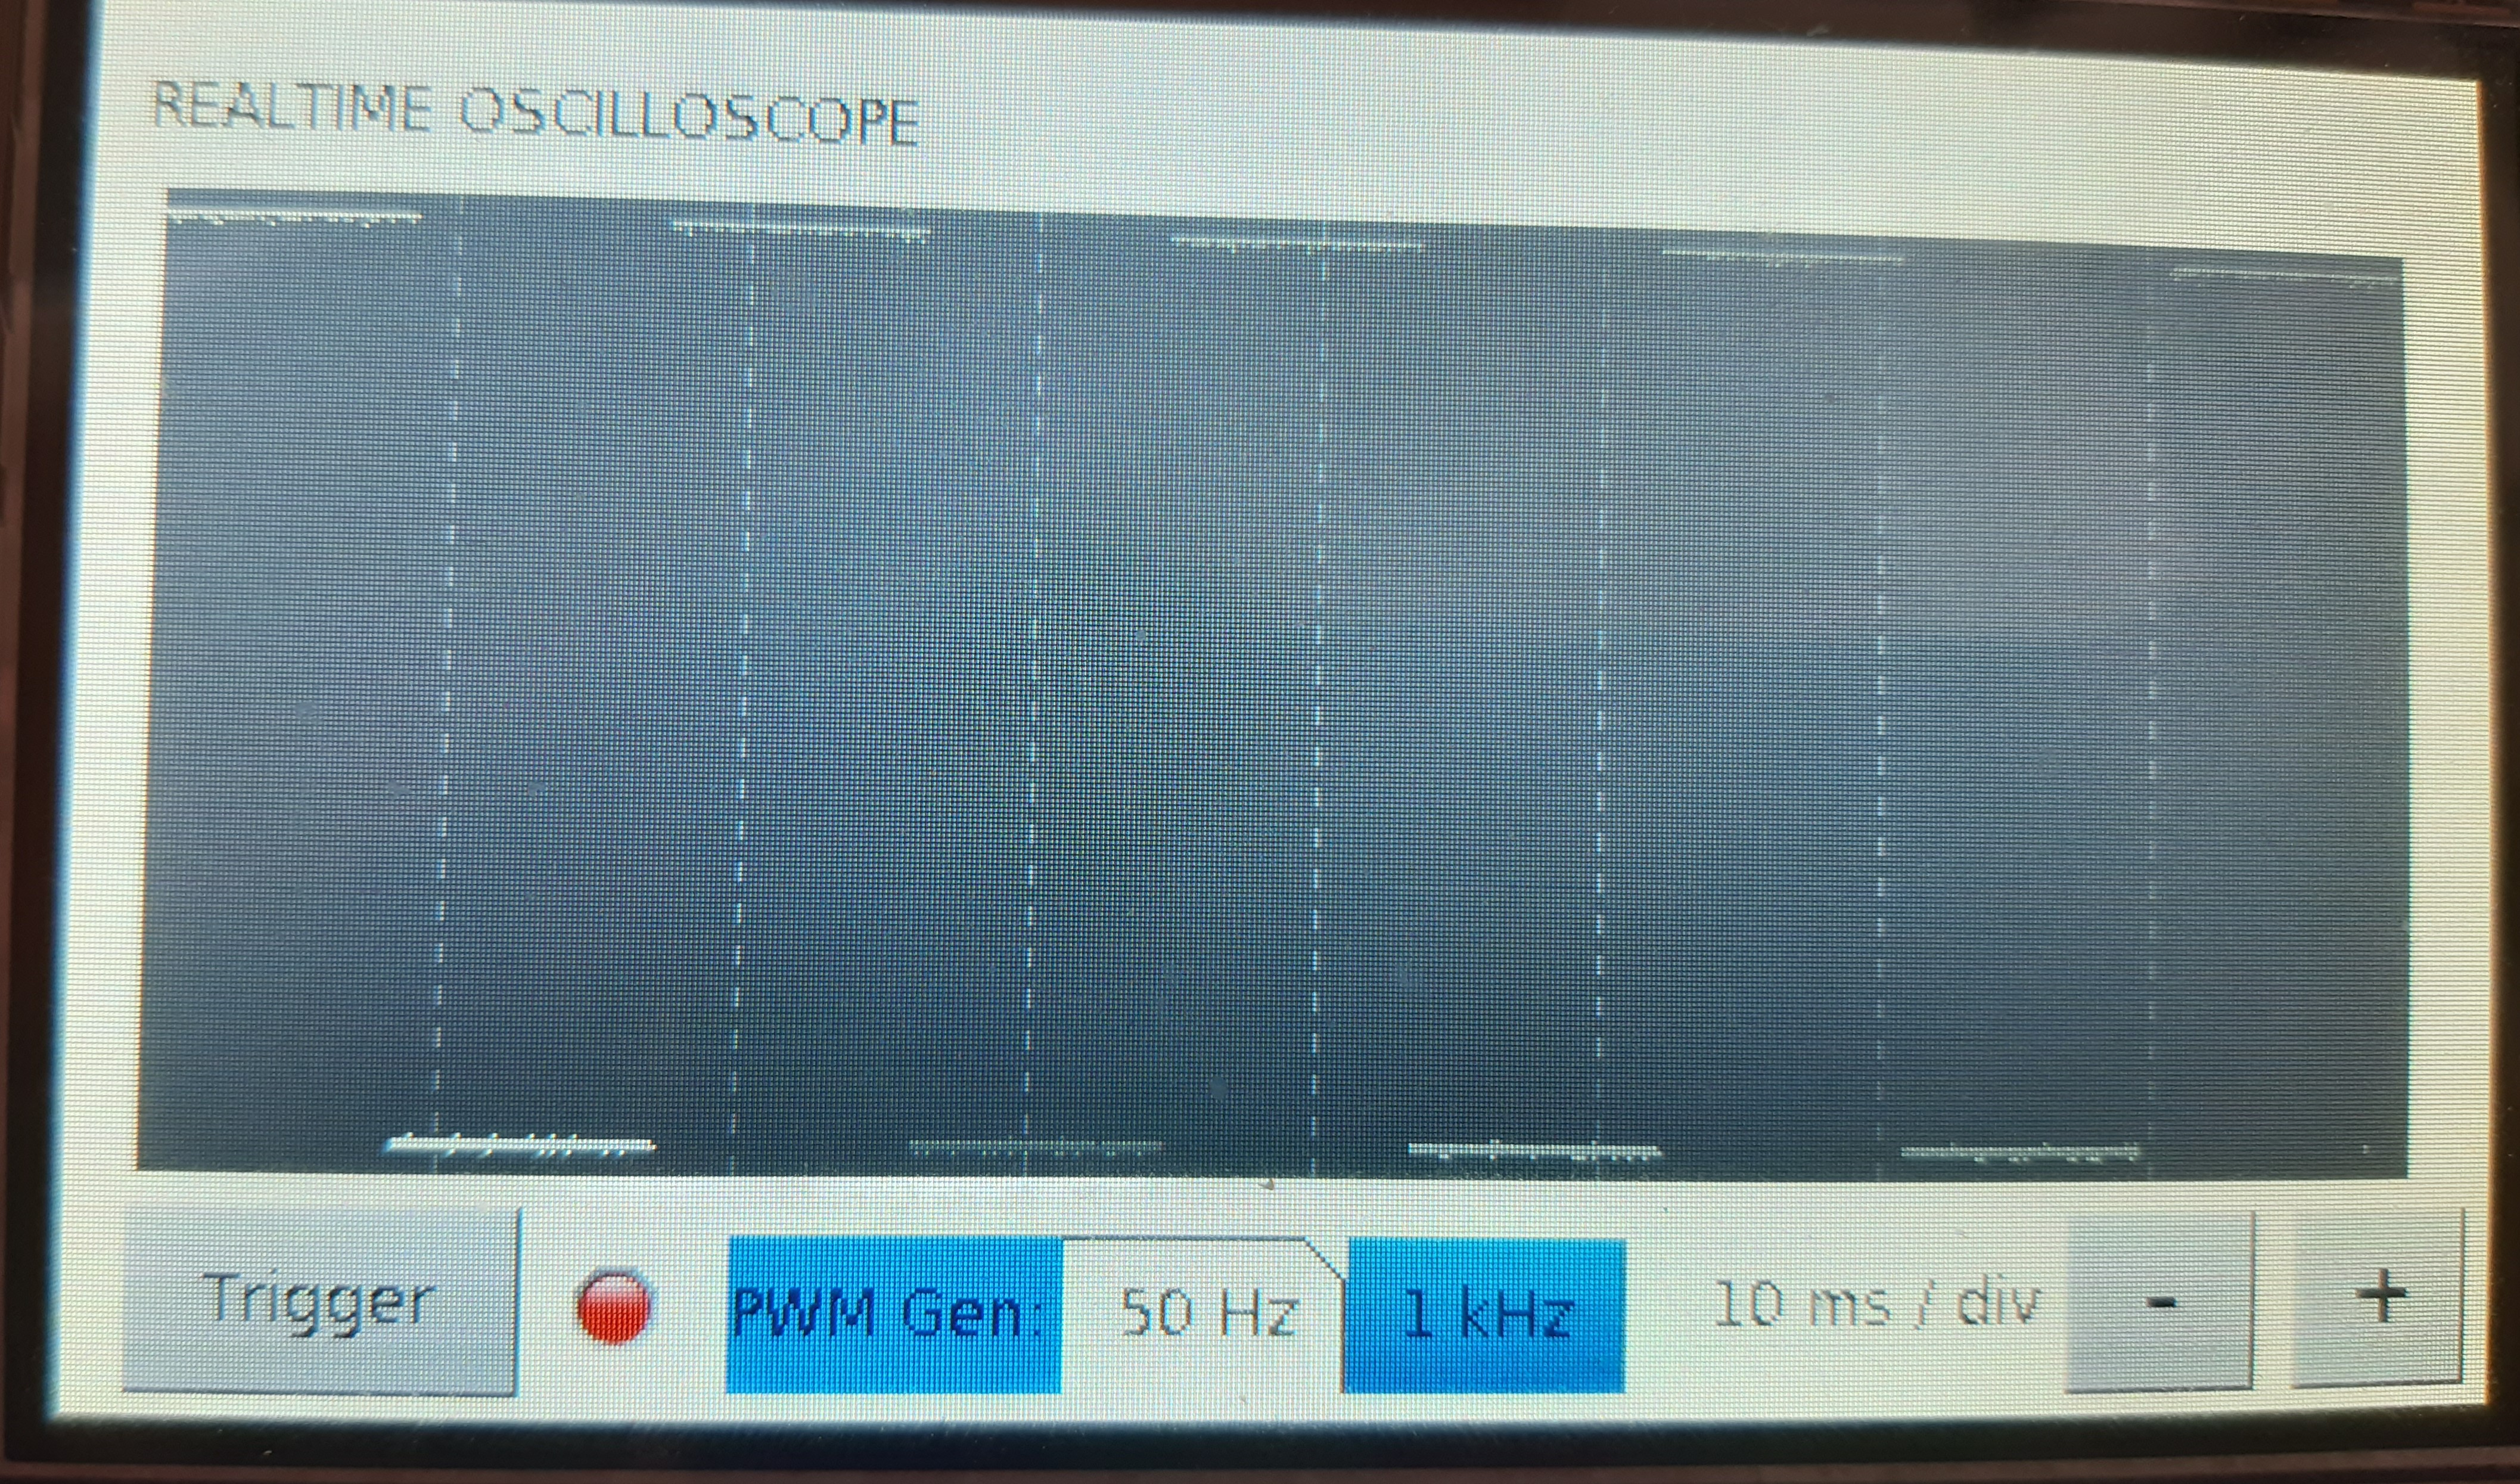
\includegraphics[scale=0.08]{Ressources/PWM_10ms}\\ 
			\hline 
			\multicolumn{2}{|c|}{Final Conditions:}&\\ 
			\hline 
			\multicolumn{2}{|c|}{Comments:}&\\ 
			\hline 
			\multicolumn{2}{|c|}{Test Passed:}&Yes \\ 
			\hline 
		\end{tabular} 
	\end{center}
\end{table}	
		\begin{table}[H]
	\begin{center}
		\begin{tabular}{| m{2cm}|m{2cm}|m{12cm}|}
			\hline 
			\bf D3&\bf Title:&\bf Check if Sinus wave can be correclty visualised\\ 
			\hline 
			\multicolumn{2}{|c|}{Group:}&Signal Display\\ 
			\hline 
			\multicolumn{2}{|c|}{Description:}&1 kHz Signal with 500 us/div time base\\ 
			\hline 
			\multicolumn{2}{|c|}{Initial Conditions:}&Sampling rate: 100kSamples/s\\ 
			\hline 
			\multicolumn{2}{|c|}{Test Results:}&The sampling frequency is high enough. There are enough points.
			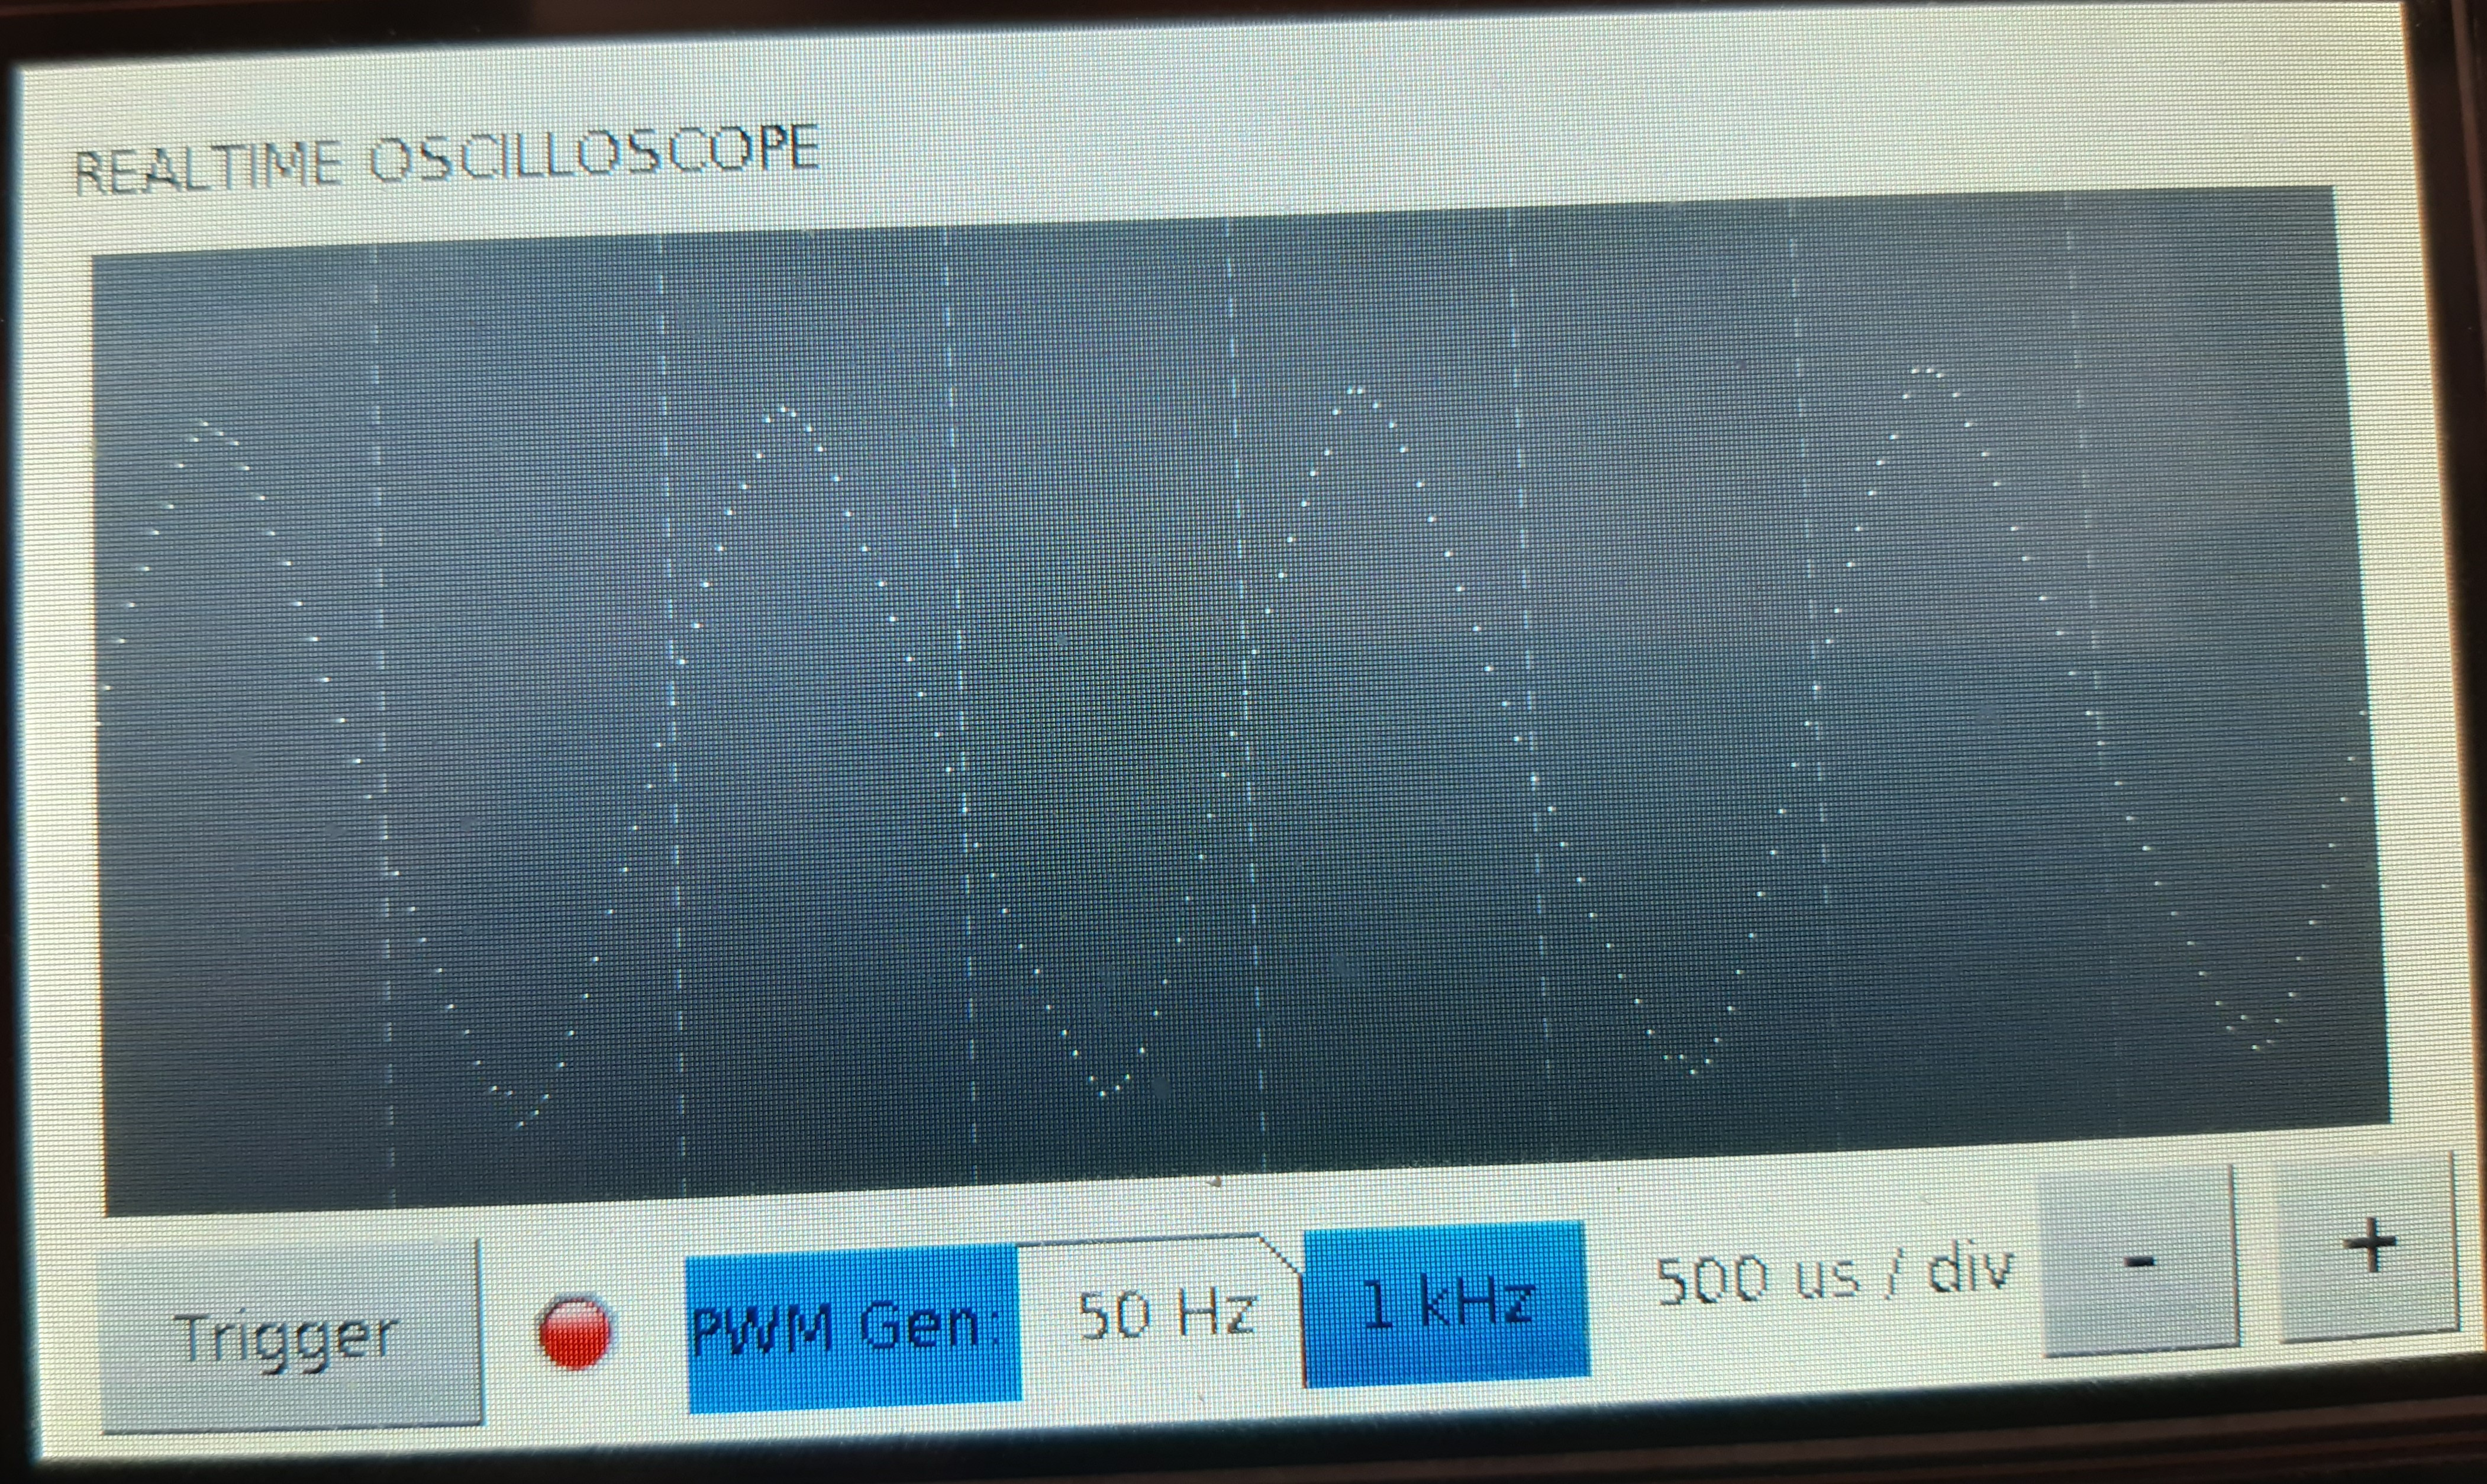
\includegraphics[scale=0.08]{Ressources/sinus_500us}\\ 
			\hline 
			\multicolumn{2}{|c|}{Final Conditions:}&\\ 
			\hline 
			\multicolumn{2}{|c|}{Comments:}&\\ 
			\hline 
			\multicolumn{2}{|c|}{Test Passed:}&Yes \\ 
			\hline 
		\end{tabular} 
	\end{center}
\end{table}	
		\begin{table}[H]
	\begin{center}
		\begin{tabular}{| m{2cm}|m{2cm}|m{12cm}|}
			\hline 
			\bf D4&\bf Title:&\bf Check if Sinus wave can be correclty visualised\\ 
			\hline 
			\multicolumn{2}{|c|}{Group:}&Signal Display\\ 
			\hline 
			\multicolumn{2}{|c|}{Description:}&1 kHz Signal with 10 ms/div time base\\ 
			\hline 
			\multicolumn{2}{|c|}{Initial Conditions:}&Sampling rate: 100kSamples/s\\ 
			\hline 
			\multicolumn{2}{|c|}{Test Results:}&The sampling frequency is high enough. There are enough points.
			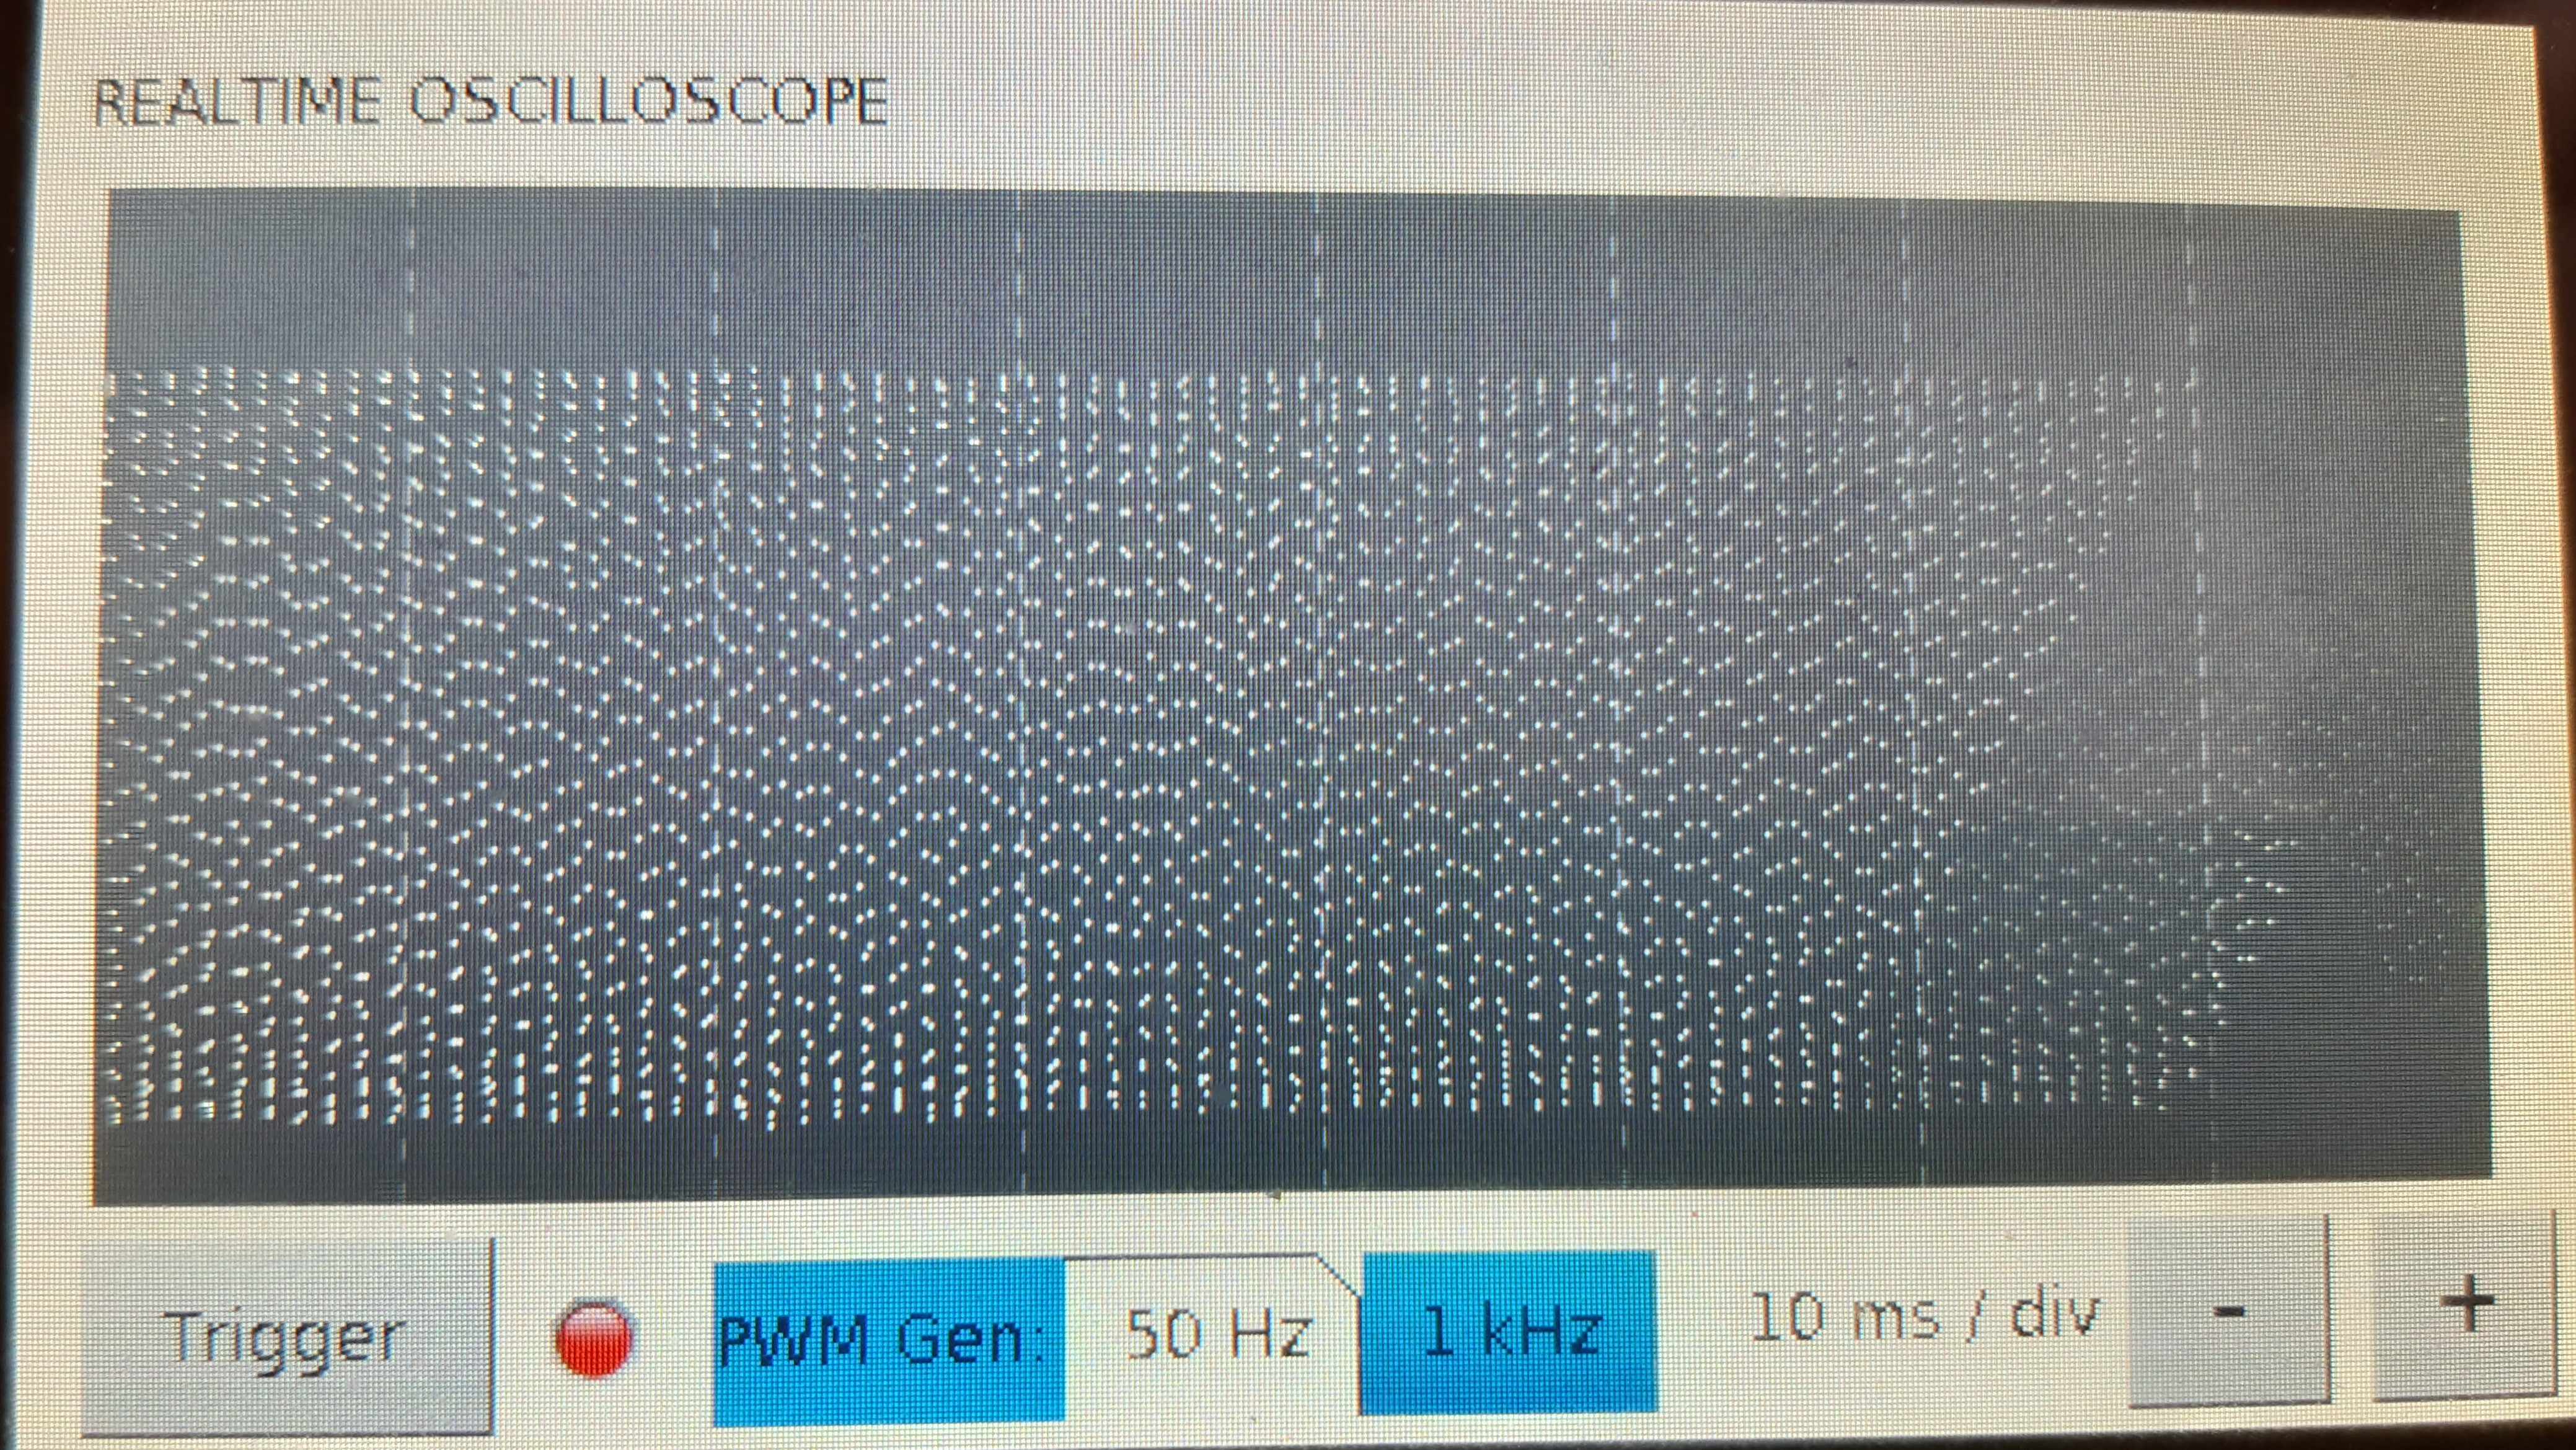
\includegraphics[scale=0.08]{Ressources/sinus_10ms}\\ 
			\hline 
			\multicolumn{2}{|c|}{Final Conditions:}&\\ 
			\hline 
			\multicolumn{2}{|c|}{Comments:}&\\ 
			\hline 
			\multicolumn{2}{|c|}{Test Passed:}&Yes \\ 
			\hline 
		\end{tabular} 
	\end{center}
\end{table}	
\subsection{E}
		\begin{table}[H]
	\begin{center}
		\begin{tabular}{| m{2cm}|m{2cm}|m{12cm}|}
			\hline 
			\bf E1&\bf Title:&\bf Check maximum display refresh rate\\ 
			\hline 
			\multicolumn{2}{|c|}{Group:}&Display Refresh Rate\\ 
			\hline 
			\multicolumn{2}{|c|}{Description:}&Display refresh rate: 50 Hz\\ 
			\hline 
			\multicolumn{2}{|c|}{Initial Conditions:}&Display refresh rate: 50 Hz\\ 
			\hline 
			\multicolumn{2}{|c|}{Test Results:}&The refresh is correctly done\\ 
			\hline 
			\multicolumn{2}{|c|}{Final Conditions:}&\\ 
			\hline 
			\multicolumn{2}{|c|}{Comments:}&\\ 
			\hline 
			\multicolumn{2}{|c|}{Test Passed:}&Yes \\ 
			\hline 
		\end{tabular} 
	\end{center}
\end{table}	
		\begin{table}[H]
	\begin{center}
		\begin{tabular}{| m{2cm}|m{2cm}|m{12cm}|}
			\hline 
			\bf E2&\bf Title:&\bf Check maximum display refresh rate\\ 
			\hline 
			\multicolumn{2}{|c|}{Group:}&Display Refresh Rate\\ 
			\hline 
			\multicolumn{2}{|c|}{Description:}&Display refresh rate: 66 Hz\\ 
			\hline 
			\multicolumn{2}{|c|}{Initial Conditions:}&Display refresh rate: 66 Hz\\ 
			\hline 
			\multicolumn{2}{|c|}{Test Results:}&The refresh is correctly done\\ 
			\hline 
			\multicolumn{2}{|c|}{Final Conditions:}&\\ 
			\hline 
			\multicolumn{2}{|c|}{Comments:}&\\ 
			\hline 
			\multicolumn{2}{|c|}{Test Passed:}&Yes \\ 
			\hline 
		\end{tabular} 
	\end{center}
\end{table}	
		\begin{table}[H]
	\begin{center}
		\begin{tabular}{| m{2cm}|m{2cm}|m{12cm}|}
			\hline 
			\bf E3&\bf Title:&\bf Check maximum display refresh rate\\ 
			\hline 
			\multicolumn{2}{|c|}{Group:}&Display Refresh Rate\\ 
			\hline 
			\multicolumn{2}{|c|}{Description:}&Display refresh rate: 100 Hz\\ 
			\hline 
			\multicolumn{2}{|c|}{Initial Conditions:}&Display refresh rate: 100 Hz\\ 
			\hline 
			\multicolumn{2}{|c|}{Test Results:}&The refresh is correctly done\\ 
			\hline 
			\multicolumn{2}{|c|}{Final Conditions:}&\\ 
			\hline 
			\multicolumn{2}{|c|}{Comments:}&There are no difference between all these tests. The measured duration of a refresh is 22 ms. 
			So the uC is refreshing all the time as fast as possible, even with the 50 Hz refresh rate.\\ 
			\hline 
			\multicolumn{2}{|c|}{Test Passed:}&Yes \\ 
			\hline 
		\end{tabular} 
	\end{center}
\end{table}	
\subsection{F}
		\begin{table}[H]
	\begin{center}
		\begin{tabular}{| m{2cm}|m{2cm}|m{12cm}|}
			\hline 
			\bf F1&\bf Title:&\bf Check if changes of x-axis scaling take effect on signal view\\ 
			\hline 
			\multicolumn{2}{|c|}{Group:}&Time Divisions Display\\ 
			\hline 
			\multicolumn{2}{|c|}{Description:}&From 500 us/div to 1 ms/div\\ 
			\hline 
			\multicolumn{2}{|c|}{Initial Conditions:}&Input signal: square 1kHz, Div: 500 us\\ 
			\hline 
			\multicolumn{2}{|c|}{Test Results:}&The signal changes accordingly\\ 
			\hline 
			\multicolumn{2}{|c|}{Final Conditions:}&Div: 1 ms\\ 
			\hline 
			\multicolumn{2}{|c|}{Comments:}&\\ 
			\hline 
			\multicolumn{2}{|c|}{Test Passed:}&Yes \\ 
			\hline 
		\end{tabular} 
	\end{center}
\end{table}	
		\begin{table}[H]
	\begin{center}
		\begin{tabular}{| m{2cm}|m{2cm}|m{12cm}|}
			\hline 
			\bf F2&\bf Title:&\bf Check if changes of x-axis scaling take effect on signal view\\ 
			\hline 
			\multicolumn{2}{|c|}{Group:}&Time Divisions Display\\ 
			\hline 
			\multicolumn{2}{|c|}{Description:}&From 1 ms/div to 2 ms/div\\ 
			\hline 
			\multicolumn{2}{|c|}{Initial Conditions:}&Input signal: square 1kHz, Div: 1 ms\\ 
			\hline 
			\multicolumn{2}{|c|}{Test Results:}&The signal changes accordingly\\ 
			\hline 
			\multicolumn{2}{|c|}{Final Conditions:}&Div: 2 ms \\ 
			\hline 
			\multicolumn{2}{|c|}{Comments:}&\\ 
			\hline 
			\multicolumn{2}{|c|}{Test Passed:}&Yes \\ 
			\hline 
		\end{tabular} 
	\end{center}
\end{table}	
		\begin{table}[H]
	\begin{center}
		\begin{tabular}{| m{2cm}|m{2cm}|m{12cm}|}
			\hline 
			\bf F3&\bf Title:&\bf Check if changes of x-axis scaling take effect on signal view\\ 
			\hline 
			\multicolumn{2}{|c|}{Group:}&Time Divisions Display\\ 
			\hline 
			\multicolumn{2}{|c|}{Description:}&From 2 ms/div to 5 ms/div\\ 
			\hline 
			\multicolumn{2}{|c|}{Initial Conditions:}&Input signal: square 1kHz, Div: 2 ms\\ 
			\hline 
			\multicolumn{2}{|c|}{Test Results:}&The signal changes accordingly\\ 
			\hline 
			\multicolumn{2}{|c|}{Final Conditions:}&Div: 5 ms\\ 
			\hline 
			\multicolumn{2}{|c|}{Comments:}&\\ 
			\hline 
			\multicolumn{2}{|c|}{Test Passed:}&Yes \\ 
			\hline 
		\end{tabular} 
	\end{center}
\end{table}	
		\begin{table}[H]
	\begin{center}
		\begin{tabular}{| m{2cm}|m{2cm}|m{12cm}|}
			\hline 
			\bf F4&\bf Title:&\bf Check if changes of x-axis scaling take effect on signal view\\ 
			\hline 
			\multicolumn{2}{|c|}{Group:}&Time Divisions Display\\ 
			\hline 
			\multicolumn{2}{|c|}{Description:}&From 5 ms/div to 10 ms/div\\ 
			\hline 
			\multicolumn{2}{|c|}{Initial Conditions:}&Input signal: square 50 Hz, Div: 5 ms\\ 
			\hline 
			\multicolumn{2}{|c|}{Test Results:}&The signal changes accordingly\\ 
			\hline 
			\multicolumn{2}{|c|}{Final Conditions:}&Div: 10 ms \\ 
			\hline 
			\multicolumn{2}{|c|}{Comments:}&\\ 
			\hline 
			\multicolumn{2}{|c|}{Test Passed:}&Yes \\ 
			\hline 
		\end{tabular} 
	\end{center}
\end{table}	
		\begin{table}[H]
	\begin{center}
		\begin{tabular}{| m{2cm}|m{2cm}|m{12cm}|}
			\hline 
			\bf F5&\bf Title:&\bf Check if changes of x-axis scaling take effect on signal view\\ 
			\hline 
			\multicolumn{2}{|c|}{Group:}&Time Divisions Display\\ 
			\hline 
			\multicolumn{2}{|c|}{Description:}&From 10 ms/div back to 5 ms/div\\ 
			\hline 
			\multicolumn{2}{|c|}{Initial Conditions:}&Input signal: square 50 Hz, Div: 10 ms\\ 
			\hline 
			\multicolumn{2}{|c|}{Test Results:}&The signal changes accordingly\\ 
			\hline 
			\multicolumn{2}{|c|}{Final Conditions:}&Div: 5 ms\\ 
			\hline 
			\multicolumn{2}{|c|}{Comments:}&\\ 
			\hline 
			\multicolumn{2}{|c|}{Test Passed:}&Yes \\ 
			\hline 
		\end{tabular} 
	\end{center}
\end{table}	
		\begin{table}[H]
	\begin{center}
		\begin{tabular}{| m{2cm}|m{2cm}|m{12cm}|}
			\hline 
			\bf F6&\bf Title:&\bf Check if changes of x-axis scaling take effect on signal view\\ 
			\hline 
			\multicolumn{2}{|c|}{Group:}&Time Divisions Display\\ 
			\hline 
			\multicolumn{2}{|c|}{Description:}&From 5 ms/div back to 2 ms/div\\ 
			\hline 
			\multicolumn{2}{|c|}{Initial Conditions:}&Input signal: square 50 Hz, Div: 5 ms\\ 
			\hline 
			\multicolumn{2}{|c|}{Test Results:}&The signal changes accordingly\\ 
			\hline 
			\multicolumn{2}{|c|}{Final Conditions:}&Div: 2 ms\\ 
			\hline 
			\multicolumn{2}{|c|}{Comments:}&\\ 
			\hline 
			\multicolumn{2}{|c|}{Test Passed:}&Yes \\ 
			\hline 
		\end{tabular} 
	\end{center}
\end{table}	
		\begin{table}[H]
	\begin{center}
		\begin{tabular}{| m{2cm}|m{2cm}|m{12cm}|}
			\hline 
			\bf F7&\bf Title:&\bf Check if changes of x-axis scaling take effect on signal view\\ 
			\hline 
			\multicolumn{2}{|c|}{Group:}&Time Divisions Display\\ 
			\hline 
			\multicolumn{2}{|c|}{Description:}&From 2 ms/div to 1 ms/div\\ 
			\hline 
			\multicolumn{2}{|c|}{Initial Conditions:}&Input signal: square 1kHz, Div: 2 ms\\ 
			\hline 
			\multicolumn{2}{|c|}{Test Results:}&The signal changes accordingly\\ 
			\hline 
			\multicolumn{2}{|c|}{Final Conditions:}&Div: 1 ms \\ 
			\hline 
			\multicolumn{2}{|c|}{Comments:}&\\ 
			\hline 
			\multicolumn{2}{|c|}{Test Passed:}&Yes \\ 
			\hline 
		\end{tabular} 
	\end{center}
\end{table}	
		\begin{table}[H]
	\begin{center}
		\begin{tabular}{| m{2cm}|m{2cm}|m{12cm}|}
			\hline 
			\bf F8&\bf Title:&\bf Check if changes of x-axis scaling take effect on signal view\\ 
			\hline 
			\multicolumn{2}{|c|}{Group:}&Time Divisions Display\\ 
			\hline 
			\multicolumn{2}{|c|}{Description:}&From 1 ms/div to 500 us/div\\ 
			\hline 
			\multicolumn{2}{|c|}{Initial Conditions:}&Input signal: square 1kHz, Div: 1 ms\\ 
			\hline 
			\multicolumn{2}{|c|}{Test Results:}&The signal changes accordingly\\ 
			\hline 
			\multicolumn{2}{|c|}{Final Conditions:}&Div: 500 us\\ 
			\hline 
			\multicolumn{2}{|c|}{Comments:}&\\ 
			\hline 
			\multicolumn{2}{|c|}{Test Passed:}&Yes \\ 
			\hline 
		\end{tabular} 
	\end{center}
\end{table}	
\subsection{G}
		\begin{table}[H]
	\begin{center}
		\begin{tabular}{| m{2cm}|m{2cm}|m{12cm}|}
			\hline 
			\bf G1-5&\bf Title:&\bf Check if when enabling signal triggering, the periodic signal stays still on the display\\ 
			\hline 
			\multicolumn{2}{|c|}{Group:}&Trigger Signal Display\\ 
			\hline 
			\multicolumn{2}{|c|}{Description:}&Enable the triggering, and change the time base\\ 
			\hline 
			\multicolumn{2}{|c|}{Initial Conditions:}&Input signal: 50Hz square, Div: 500us\\ 
			\hline 
			\multicolumn{2}{|c|}{Test Results:}&The periodic signal stay still on the display, but sometimes it moves just for 1 frame.\\ 
			\hline 
			\multicolumn{2}{|c|}{Final Conditions:}&Div: 10 ms\\ 
			\hline 
			\multicolumn{2}{|c|}{Comments:}&\\ 
			\hline 
			\multicolumn{2}{|c|}{Test Passed:}&Partially \\ 
			\hline 
		\end{tabular} 
	\end{center}
\end{table}	
		\begin{table}[H]
	\begin{center}
		\begin{tabular}{| m{2cm}|m{2cm}|m{12cm}|}
			\hline 
			\bf G6-10&\bf Title:&\bf Check if when enabling signal triggering, the periodic signal stays still on the display\\ 
			\hline 
			\multicolumn{2}{|c|}{Group:}&Trigger Signal Display\\ 
			\hline 
			\multicolumn{2}{|c|}{Description:}&Enable the triggering, and change the time base\\ 
			\hline 
			\multicolumn{2}{|c|}{Initial Conditions:}&Input signal: 1kHz triangle, Div: 500us\\ 
			\hline 
			\multicolumn{2}{|c|}{Test Results:}&The periodic signal stay still on the display, but sometimes it moves just for 1 frame.\\ 
			\hline 
			\multicolumn{2}{|c|}{Final Conditions:}&Div: 10 ms\\ 
			\hline 
			\multicolumn{2}{|c|}{Comments:}&\\ 
			\hline 
			\multicolumn{2}{|c|}{Test Passed:}&Partially \\ 
			\hline 
		\end{tabular} 
	\end{center}
\end{table}	
		\begin{table}[H]
	\begin{center}
		\begin{tabular}{| m{2cm}|m{2cm}|m{12cm}|}
			\hline 
			\bf G11-15&\bf Title:&\bf Check if when enabling signal triggering, the periodic signal stays still on the display\\ 
			\hline 
			\multicolumn{2}{|c|}{Group:}&Trigger Signal Display\\ 
			\hline 
			\multicolumn{2}{|c|}{Description:}&Enable the triggering, and change the time base\\ 
			\hline 
			\multicolumn{2}{|c|}{Initial Conditions:}&Input signal: 1kHz sinus, Div: 500us\\ 
			\hline 
			\multicolumn{2}{|c|}{Test Results:}&The periodic signal stay still on the display, but sometimes it moves just for 1 frame.\\ 
			\hline 
			\multicolumn{2}{|c|}{Final Conditions:}&Div: 10 ms\\ 
			\hline 
			\multicolumn{2}{|c|}{Comments:}&\\ 
			\hline 
			\multicolumn{2}{|c|}{Test Passed:}&Partially \\ 
			\hline 
		\end{tabular} 
	\end{center}
\end{table}	

\subsection{L}
		\begin{table}[H]
	\begin{center}
		\begin{tabular}{| m{2cm}|m{2cm}|m{12cm}|}
			\hline 
			\bf L1&\bf Title:&\bf Does the software hang after a while?\\ 
			\hline 
			\multicolumn{2}{|c|}{Group:}&Long-Term Test\\ 
			\hline 
			\multicolumn{2}{|c|}{Description:}&Check if the system is running without user interaction for about 5 minutes\\ 
			\hline 
			\multicolumn{2}{|c|}{Initial Conditions:}&With RTOS\\ 
			\hline 
			\multicolumn{2}{|c|}{Test Results:}&The system still run correctly\\ 
			\hline 
			\multicolumn{2}{|c|}{Final Conditions:}&\\ 
			\hline 
			\multicolumn{2}{|c|}{Comments:}&\\ 
			\hline 
			\multicolumn{2}{|c|}{Test Passed:}&Yes \\ 
			\hline 
		\end{tabular} 
	\end{center}
\end{table}	
		\begin{table}[H]
	\begin{center}
		\begin{tabular}{| m{2cm}|m{2cm}|m{12cm}|}
			\hline 
			\bf L2&\bf Title:&\bf Does the software hang after a while?\\ 
			\hline 
			\multicolumn{2}{|c|}{Group:}&Long-Term Test\\ 
			\hline 
			\multicolumn{2}{|c|}{Description:}&Check if system is running with continuous user interaction for about 5 minutes\\ 
			\hline 
			\multicolumn{2}{|c|}{Initial Conditions:}&With RTOS\\ 
			\hline 
			\multicolumn{2}{|c|}{Test Results:}&The system still run correctly\\ 
			\hline 
			\multicolumn{2}{|c|}{Final Conditions:}&\\ 
			\hline 
			\multicolumn{2}{|c|}{Comments:}&\\ 
			\hline 
			\multicolumn{2}{|c|}{Test Passed:}&Yes \\ 
			\hline 
		\end{tabular} 
	\end{center}
\end{table}	
		\begin{table}[H]
	\begin{center}
		\begin{tabular}{| m{2cm}|m{2cm}|m{12cm}|}
			\hline 
			\bf L3&\bf Title:&\bf Does the software hang after a while?\\
			\hline 
			\multicolumn{2}{|c|}{Group:}&Long-Term Test\\ 
			\hline 
			\multicolumn{2}{|c|}{Description:}&Check if system is running for more then 6 hours\\ 
			\hline 
			\multicolumn{2}{|c|}{Initial Conditions:}&With RTOS\\ 
			\hline 
			\multicolumn{2}{|c|}{Test Results:}&The system still run correctly\\ 
			\hline 
			\multicolumn{2}{|c|}{Final Conditions:}&\\ 
			\hline 
			\multicolumn{2}{|c|}{Comments:}&\\ 
			\hline 
			\multicolumn{2}{|c|}{Test Passed:}&Yes \\ 
			\hline 
		\end{tabular} 
	\end{center}
\end{table}	

\subsection{Summary}

			\begin{table}[H]
		\begin{center}
			\begin{tabular}{| m{6cm}|m{2cm}|}
				\hline 
				\bf Total Tests:&\bf 31\\
				\hline 
				Tests passed:&27\\ 
				\hline 
				Tests partially passed:&3\\ 
				\hline 
				Tests not passed:&1\\ 
				\hline 
			\end{tabular} 
		\end{center}
	\end{table}	

	\section{Conclusion}

\end{document}
